%!TEX root = virtual-clusters.tex

\section{Cloudmesh Client}

The cloudmesh client toolkit \cite{www-cloudmesh} is a lightweight
client interface for accessing heterogeneous clouds, clusters, and
workstations right from the users computer. 

The user can manage his own set of resources he utilizes providing a
personalized cyber infrastructure. Cloudmesh client includes an API, a
commandline client, and a commandline shell. It includes a the ability
to integrate new cyberinfrastuctures by providing convenient
abstractions to integrate with them. In addition it includes a local
database allowing caching of information typically retrieved from the
available infrastructure. This cache is especially useful for large
scientific workflows and services that require the management of many
tasks.  Via these attractions it is also possible to easily switch
between or utilize together virtual machines from OpenStack, Amazon,
Azure Clouds, and comet virtual clusters.  Cloudmesh client can be
installed on Linux, MacOSX, and even Windows.  Currently we support
backends to SLURM, SSH, OpenStack. In the past we supported AWS and
Azure which we are integrating back into the client.

Next we summarize the main properties of the cloudmesh client:

{\parindent 0pt \bf Client based.} Cloudmesh client as the name indicates is a client based toolkit that is installed and run on the users computers. This also includes an add on component to the cloudmesh client which is a portal. Hence we distinguish the client that contains most of the functionality, as well as a portal that can access the functionality through a locally maintaine Web portal. Important to note is that the user manages its own credentials and thus security and credential management is done directly on the users machine instead through a hosted Web portal. This increases the security as access to any credential is managed by the user and is not part of a credential management system.

{\parindent 0pt \bf Layered Architecture.} Cloudmesh client has a layered architecture that
allows easy development of new features. This also allows contribution
by the community while developing integrated and smaller sub
components. Figure A depicts the various layers. A resource
abstraction layer allows the integration of a multitude of resources
spanning HPC, Containers, and Cloud resources. (At this time we focus
on Openstack and Slurm resources. We are working on reintegrating
resources such as Azure, AWS, Maui, Moab, and others which we
previously supported, as well as new resources such as docker).

\begin{figure}[!h] 
  \centering 
    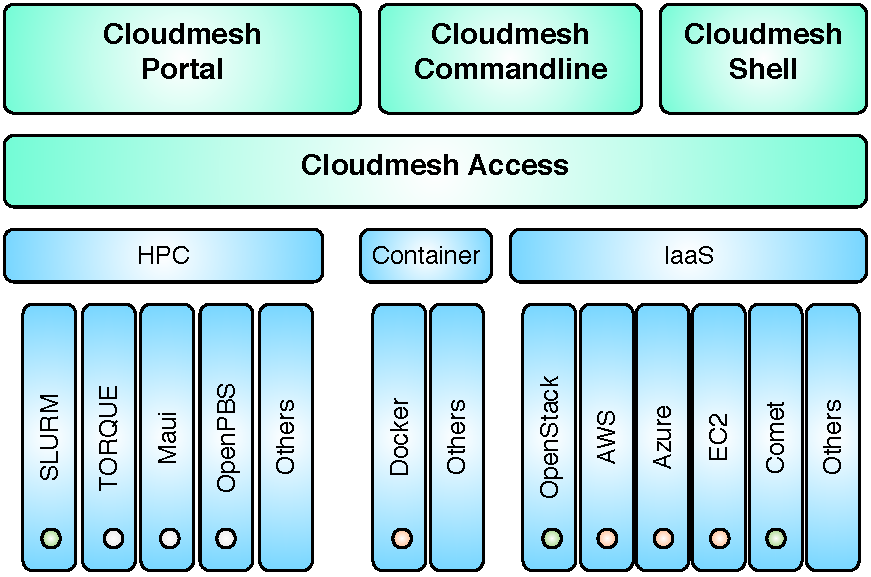
\includegraphics[width=1.0\columnwidth]{images/client/cloudmesh-arch-1.pdf} 
    \caption{Cloudmesh layered architecture.}
    \label{F:arch-1}
\end{figure} 

\begin{figure}[!h] 
  \centering 
    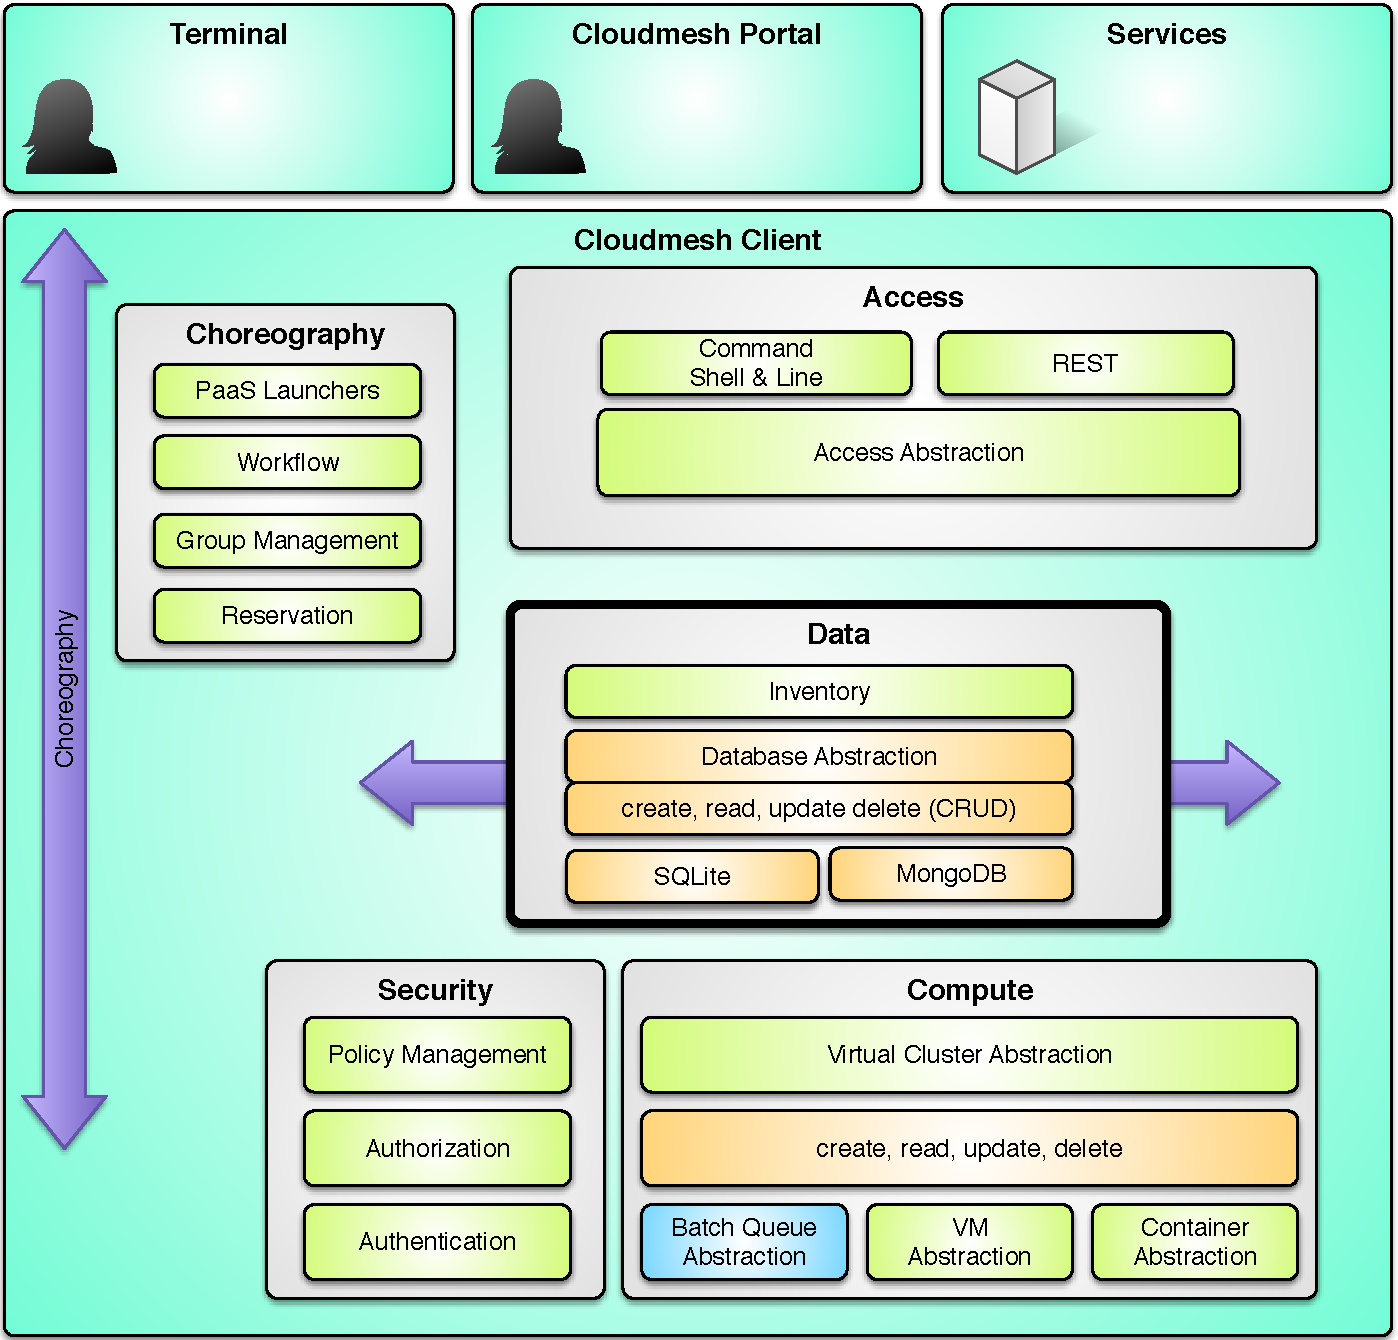
\includegraphics[width=1.0\columnwidth]{images/client/cloudmesh-arch-2.pdf} 
    \caption{Cloudmesh component overview}
    \label{F:arch-2}
\end{figure} 

\parindent 0pt { \bf Management Framework.} Cloudmesh client contains a management framework, and its components are depicted in Figure B. cloudmesh allows easy management of virtual machines, containers, and the data associated with them. We are currently developing a choreography framework that leverages Ansible, chef, and heat. All of the functionality is easily usable through a command shell that also can be used from the commandline, and a Python API. IN future we will be providing a REST API.

\parindent 0pt { \bf Database Agnostic.} Cloudmesh contains some state about the resource and environment that a user may want to use. The information is managed in an database abstraction that would allow storing the data in a variety of databases such as SQL and MongoDB. At this time we have chosen SQLite to be the default database as it does not require any additional setup and is universally available on all operating systems without change.

\parindent 0pt { \bf Command shell and line.} Cloudmesh contains a command shell allowing scripts to be developed and run. However we designed the command shell in such a way that each command can also be called from the command line. Through the cloudmesh state machine the state between command shell, command client, and the portal is shared.

\parindent 0pt { \bf Cloudmesh Client Portal.} Previously, we distributed cloudmesh with client, server, and a portal components in one package. This however turned out to be to complex to be installed for some of our less technically skilled user community. Thus we split up the install into two independent packages. The cloudmesh client and the cloudmesh portal. The portal provides some elementary features to manage virtual machines and HPC jobs. At this time the portal is considered to be alpha technology. Just as the client the portal is to be run on the local user machine in oredr to allow increased security by managing the credentials locally rather than on a server.

\parindent 0pt { \bf Cloudmesh Two Factor Authentication.} We have an exploratory project in place that looks at the use of Yubikeys for cloudmesh, client and cloudmesh portal.

\parindent 0pt { \bf Cloudmesh Comet.} We are actively developing the client interface for SDSC's comet supercomputer allowing bare metal provisioning. The interface reuses cloudmesh components and technologies while interfacing with the comet cloud REST interface. The goal here is to manage virtual clusters.


\section{Client other}


\begin{description}
\item[REST API]
\item[Command line interface]
\item[Command shell for scripting]
\item[Console Access]
\item[Portal]
\end{description}

selected commands:


\begin{figure}[htb] 

{\tt cm comet cluster  ID}\newline -- Show the cluster details

{\tt cm comet power on ID vm-ID -[0-3] --walltime=6h}\newline -- Power 3 nodes
on for 6 hours

{\tt cm comet image attach image.iso ID vm-ID-0}\newline -- Attach an image

{\tt cm comet boot ID vm-ID-0}\newline
-- Boot node 0

{\tt cm comet console vc4}\newline
-- open the console 

\end{figure}


\begin{figure}[!h] 
  \centering 
    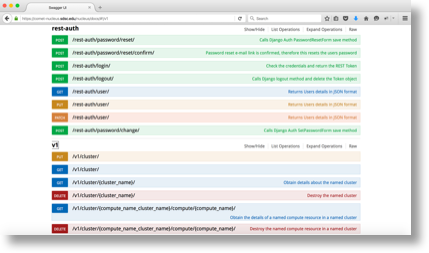
\includegraphics[width=1.0\columnwidth]{images/client/Picture1.png} 
    \caption{Rest Interface}
    \label{F:1}
%\end{figure} 

%\begin{figure}[htb] 
  \centering 
    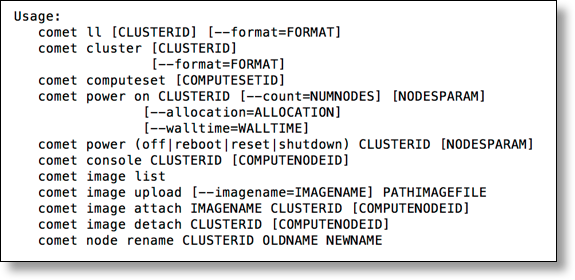
\includegraphics[width=1.0\columnwidth]{images/client/Picture2.png} 
    \caption{Commandline }
    \label{F:2}
%\end{figure} 

%\begin{figure}[htb] 
  \centering 
    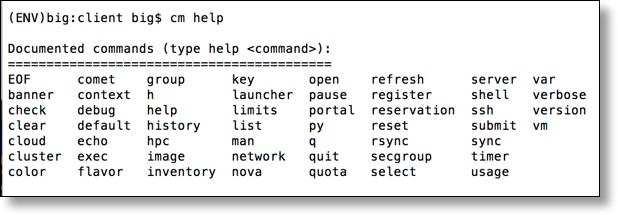
\includegraphics[width=1.0\columnwidth]{images/client/Picture3.png} 
    \caption{Command Shell}
    \label{F:3}
%\end{figure} 

\begin{comment}
\begin{figure}[htb] 
  \centering 
    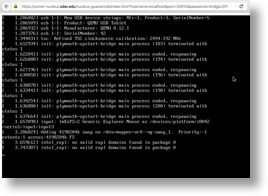
\includegraphics[width=1.0\columnwidth]{images/client/Picture4.png} 
    \caption{4}
    \label{F:4}
\end{figure} 
\end{comment}

%\begin{figure}[htb] 
  \centering 
    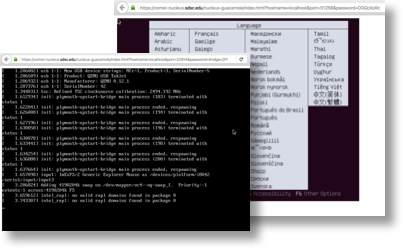
\includegraphics[width=1.0\columnwidth]{images/client/Picture5.png} 
    \caption{Console}
    \label{F:5}
\end{figure} 

\begin{figure}[htb]
\begin{tiny}
\begin{verbatim}
comet init
comet ll [CLUSTERID] [--format=FORMAT]
comet cluster [CLUSTERID][--format=FORMAT]
comet computeset [COMPUTESETID][--allocation=ALLOCATION][--cluster=CLUSTERID] 
                               [--state=COMPUTESESTATE]
comet start CLUSTERID [--count=NUMNODES][COMPUTENODEIDS][--allocation=ALLOCATION]
                      [--walltime=WALLTIME]
comet terminate COMPUTESETID
comet power (on|off|reboot|reset|shutdown) CLUSTERID [NODESPARAM]
comet console CLUSTERID [COMPUTENODEID]
comet iso list
comet iso upload [--isoname=ISONAME] PATHISOFILE
comet iso attach ISONAME CLUSTERID [COMPUTENODEIDS]
comet iso detach CLUSTERID [COMPUTENODEIDS]
comet node rename CLUSTERID OLDNAME NEWNAME

Options:
  --format=FORMAT         Format is either table, json, yaml, csv, rest [default: table]
                            
  --count=NUMNODES        Number of nodes to be powered on. When this option is used, the 
                          comet system will find a NUMNODES number of arbitrary nodes that 
                          are available to boot as a computeset
  --allocation=ALLOCATION  Allocation to charge when power on node(s)
  --walltime=WALLTIME     Walltime requested for the node(s). Walltime could be an integer 
                          value followed by a unit (m, h, d, w, for minute, hour, day,
                          and week, respectively). E.g., 3h, 2d
  --isoname=ISONAME       Name of the iso image after being stored remotely. If not specified, 
                          use the original filename
  --state=COMPUTESESTATE  List only computeset with the specified state. The state could be 
                          submitted, running, completed
Arguments:
  CLUSTERID       The assigned name of a cluster, e.g. vc1
  COMPUTESETID    An integer identifier assigned to a computeset
  COMPUTENODEID   A compute node name, e.g., vm-vc1-0
                  If not provided, the requested action will be taken
                  on the frontend node of the specified cluster
  COMPUTENODEIDS  A set of compute node names in hostlist format, e.g., vm-vc1-[0-3]
                  One single node is also acceptable: vm-vc1-0. If not provided, the requested 
                  action will be taken on the frontend node of the specified cluster
  NODESPARAM      Specifying the node/nodes/computeset to act on. In case of integer, will 
                  be intepreted as a computesetid; in case of a hostlist format, 
                  e.g., vm-vc1-[0-3], a group of nodes; or a single host is also acceptable,
                  e.g., vm-vc1-0
  ISONAME         Name of an iso image at remote server
  PATHISOFILE     The full path to the iso image file to be uploaded
\end{verbatim}
\end{tiny}
\caption{Manual Page}\label{F:man}
\end{figure}


\subsection{Hybrid Cloud Achievement}


Comet has easy to use CLI allowing the use of Comet as infrastructure
for virtual cluster management.


Cloudmesh has more functionality:
\begin{itemize}
\item Access hybrid clouds OpenStack, (EC2, AWS, Azure) Access
  concrete
\item infrastructure demonstrated usages of FutureSystems, Chameleon,
\item CloudLab, Cybera (CA) Once we get access: Bridges, Jetstream, ...
\item (EC2, AWS, Azure)
\end{itemize}
A user could use all of them

\subsection{Motivation}

Users are flexible and can chose the infrastructure most suitable for
a particular problem while accessing them through the same client.
Switching from one infrastructure to another is simple while using
templates and defaults

\begin{verbatim}
cm var cloud=jetstream / bridges / aws / ...
cm default cloud=$cloud
cm boot
\end{verbatim}

Rich Platform Stacks to Enable Reusable Virtual Cluster Templates

\begin{itemize}
\item Leverage from open source and proprietary services and tools
\item Pick the one most suitable
\item Integrate in DevOps
\item Make available through Cloudmesh launchers
\end{itemize}
cloudmesh launcher

Example:Install a Compute Node


\subsection{Virtual Clusters}

\begin{itemize}
\item Successful Early Operations
\item Developed a functional cloud environment leveraging:
\item Existing Rocks virtual cluster features
\item IU's FutureGrid experience and Cloudmesh client
\item Our ability to integrate with the standard HPC environment
\item Successfully deployed OSG virtual cluster
\item Virtual cluster used for CAIDA BGP Hackathon 2016
\item Hardening features
\item On ramping new groups
\item Pushing virtual cluster capability further into Comet
\item Excitement and caution
\item Developing cluster templates (Generic HPC cluster, Big Data) via Cloudmesh Launchers
\end{itemize}

\subsection{Other achievements}
\begin{itemize}
\item Pioneering XSEDE Cloud Allocation and Accounting
\item Virtual clusters use compute nodes as building blocks
\item Allocated based on compute SUs
\item Usage tracked based on compute SUs
\item XDMoD adding cloud utilization features via Open XDMoD
\item Builds on hardware resource utilization from TACC Stats
\item Needed for Comet, Jetstream, future XSEDE cloud systems
\item Need to have ongoing conversation with early users about \item reporting
\item Should projects report back like gateways?
\item Users, jobs, etc.?
\item Projects will likely need to track for subsequent XRACs \item regardless
\item After OSG, Many New Projects Ready to Begin
\item User-Customized HPC
\item High Performance Virtual Cluster Characteristics
\item What About Data?
\item Local storage
\item Can use Seagate SSDs for large VM images
\item Local (SDSC) network access same as compute nodes
\item We provide modest (TB) storage via NFS now
\item Working on secure access to Lustre
\item Accessing Virtual Cluster Capabilities
\end{itemize}



\subsection{What is next: Platforms}

\begin{itemize}
\item Example: NIST BigData Working group
\item Gather use case input from all stakeholders 
\item Derive Big Data requirements from each use case.
\item Analyze/prioritize a list of challenging general requirements that may delay or prevent adoption of BigData deployment 
\item Work with Reference Architecture to validate requirements and reference architecture
\item Develop a set of general patterns capturing the {\em essence} of use cases (to do)
\item Rich Platform Stacks to Enable Reusable Virtual Cluster Templates
\item Leverage from open source and proprietary services and tools
\item Pick the one most suitable
\item Integrate in DevOps
\item Make available through Cloudmesh launchers
\end{itemize}

\subsection{Comet Cloudmesh Platform Launchers}

\begin{itemize}
\item Launch specific platform selections
\item Target Application user communities
\item Make deployment and management simple
\item Customizable launchers
\item Launchers available through commandline or browser
\item Underlying ZFS layer makes cloning cluster template trivial
\item Comet Cloudmesh Platform Launchers (Future)
\item Specific Launch
\item List of Launchers
\item Concepts, Ideas, Design
\end{itemize}

\subsection{Enabling Technologies}
\begin{description}
\item[KVM:] Let us run virtual machines (all processor features)
\item[SR-IOV:] Makes MPI go fast on VMs
\item[Rocks:] Systems management
\item[ZFS:] Disk image management
\item[VLANs:] Isolate virtual cluster management network
\item[pkeys:] Isolate virtual cluster IB network
\item[Nucleus:] Coordination engine (scheduling, provisioning, status,
  etc.)
\item[Cloudmesh:] The client to virtual cluster management is
  provided by cloudmesh 
\end{description}


\subsection{User Perspective}

51 NIST Big Data Benchmark Detailed Use Cases

\begin{description}
\item [Government Operation:] National Archives and Records
  Administration, Census BureauCommercial: Finance in Cloud, Cloud
  Backup, Mendeley (Citations), Netfilx, Web Search, Digital
  Materials, Cargo shipping (as in UPS)Defense: Sensors, Image
  surveillance, Situation AssessmentHealthcare and
\item[Life Sciences:] Medical records, Graph and Probabilistic
  analysis, Pathology, Bioimaging, Genomics, Epidemiology, People
  Activity models, BiodiversityDeep Learning and Social Media: Driving
  Car, Geolocate images/cameras, Twitter, Crowd Sourcing, Network
  Science, NIST benchmark datasets
\item[The Ecosystem for Research:] Metadata, Collaboration, Language
  Translation, Light source experiments
\item[Astronomy and Physics:] Sky Surveys compared to simulation,
  Large Hadron Collider at CERN, Belle Accelerator II in JapanEarth,
\item[Environmental and Polar Science:] Radar Scattering in
  Atmosphere, Earthquake, Ocean, Earth Observation, Ice sheet Radar
  scattering, Earth radar mapping, Climate simulation datasets,
  Atmospheric turbulence identification, Subsurface Biogeochemistry
  (microbes to watersheds), AmeriFlux and FLUXNET gas sensors
\item[Energy:] SmartGrid infrastructure for virtual cluster management.
\end{description}



\begin{verbatim}
http://cloudmesh.github.io/client/reference_card.html#refcard-comet
http://cloudmesh.github.io/client/commands/command_comet.html#comet-command
\end{verbatim}

\subsection{Installation and Configuration}

The cloudmesh client is easy to install. It is available via
pip\footnote{pip installation will be available by the time this paper
  will be published.} and as source package hosted on
github.com\footnote{git clone
  https://github.com/cloudmesh/client.git}. Important for the
development of the client was from the beginning on that it is
supported in Python 2.7 and Python 3.5. The pip installation is
recommended to be conducted in pythons {\em virtualenv}.

To add configuration information the client has a special {\em init}
command that queries the user for needed input such as username and
project number, as well as setting up the authentication method. This
configuration has only to be performed once.

\subsection{Client Portal}

\begin{figure}[htb] 
  \centering 
    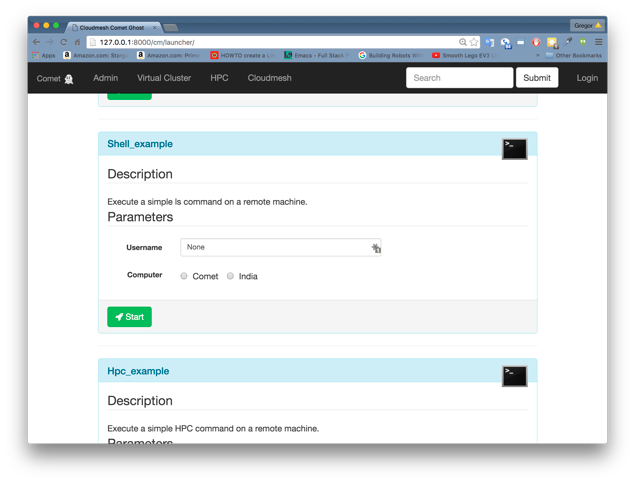
\includegraphics[width=1.0\columnwidth]{images/client/Picture6.png} 
    \caption{Virtual cluster launch parameters}
    \label{F:6}
\end{figure} 

\begin{figure}[htb] 
  \centering 
    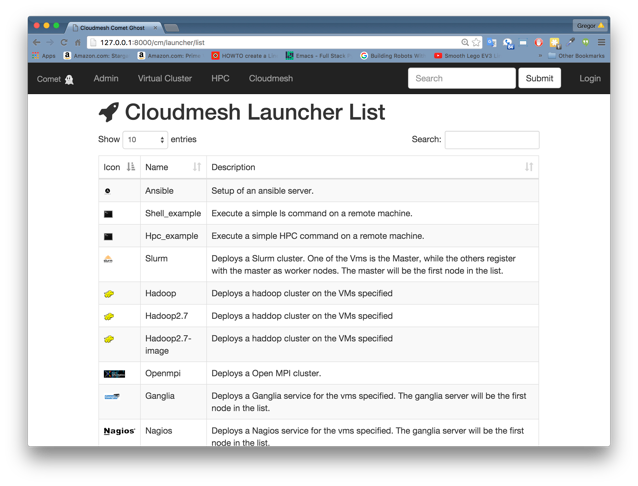
\includegraphics[width=1.0\columnwidth]{images/client/Picture7.png} 
    \caption{Virtual cluster launcher}
    \label{F:7}
\end{figure} 


\begin{comment}

\subsection{Form Tutorial}

\begin{figure*}[htb] 
\begin{small}
\begin{verbatim}

+------+---------+-------+------------------------------------------+---------------+------------+-----------+-------------+
| Name | Project | Count | Nodes                                    | Frontend (Fe) | State (Fe) | Type (Fe) | Description |
+------+---------+-------+------------------------------------------+---------------+------------+-----------+-------------+
| vc1  | sys200  | 8     | vc1-[0-7]                                | vc1           | nostate    | VM        |             |
| vc2  | iu      | 8     | vm-vc2-[0-7]                             | vc2           | active     | VM        |             |
| vc3  | sys200  | 16    | compute-0-[0-12,14],compute_windows_10,d | vc3           | active     | VM        |             |
|      |         |       | imm_dev_node                             |               |            |           |             |
| vc4  | iu      | 8     | tstfw[1-2],vm-vc4-[0-5]                  | vc4           | active     | VM        |             |
| vc5  | sys200  | 11    | vm-vc5-[0-10]                            | vc5           | nostate    | VM        |             |
| vc6  | rocks   | 8     | vm-vc6-[0-7]                             | vc6           | nostate    | VM        |             |
| vc8  | sys200  | 0     |                                          | vc8           | active     | VM        |             |
| osg  | osg     | 34    | vm-osg-[0-33]                            | osg           | active     | VM        |             |
+------+---------+-------+------------------------------------------+---------------+------------+-----------+-------------+
\end{verbatim}
\end{small}
\end{figure*}

\begin{figure*}[htb] 
\begin{small}
\begin{verbatim}

Comet Cloudmesh Client (cluster view)
(COMET)host:client$ cm comet cluster
Cluster: osg	Frontend: osg	IP: 10.21.255.180
Cluster: vc1	Frontend: vc1	IP: 10.21.255.182
.........
Cluster: vc8	Frontend: vc8	IP: 10.21.255.175
\end{verbatim}
\end{small}
\end{figure*}

\begin{figure*}[htb] 
\begin{small}
\begin{verbatim}


+--------------------+---------------+----------+------+-------------------+------+---------+--------+---------+------------+
| name               | state         | kind     | type | mac               | cpus | cluster | RAM(M) | disk(G) | computeset |
+--------------------+---------------+----------+------+-------------------+------+---------+--------+---------+------------+
| osg                | active        | frontend | VM   | ca:5f:a8:00:00:1b | 8    | osg     | 32768  | 36      |            |
|                    |               |          |      | ca:5f:a8:00:00:1c |      |         |        |         |            |
| vm-osg-0           | active        | compute  | VM   | ca:5f:a8:00:00:1d | 24   | osg     | 120000 | 100     | 1065       |
| vm-osg-1           | active        | compute  | VM   | ca:5f:a8:00:00:1e | 24   | osg     | 120000 | 100     | 1066       |
| vm-osg-2           | active        | compute  | VM   | ca:5f:a8:00:00:1f | 24   | osg     | 120000 | 100     | 1067       |
.........
| vm-vc6-6           | nostate       | compute  | VM   | ca:5f:a8:00:00:7a | 24   | vc6     | 120000 | 36      |            |
| vm-vc6-7           | nostate       | compute  | VM   | ca:5f:a8:00:00:7b | 24   | vc6     | 120000 | 36      |            |
| vc8                | active        | frontend | VM   | ca:5f:a8:00:00:6d | 2    | vc8     | 4096   | 160     |            |
|                    |               |          |      | ca:5f:a8:00:00:6e |      |         |        |         |            |
+--------------------+---------------+----------+------+-------------------+------+---------+--------+---------+------------+
\end{verbatim}
\end{small}
\end{figure*}

\begin{figure*}[htb] 
\begin{small}
\begin{verbatim}


Comet Cloudmesh Client (computeset view)
(COMET)host:client$ cm comet computeset --cluster=osg

ClusterID: osg	ComputesetID: 1065	 State: running		Allocation: sys200
Start (est): 03/29/16 16:55 EDT		End (est): 03/31/16 16:55 EDT
Requested Time (ddd-hh:mm): 2-00:00	Running Time (est): 1-19:23		Remaining Time (est): 04:36
+----------+--------+------+-------------------+------+---------+------+--------+
| name     | state  | type | mac               | cpus | cluster | host | memory |
+----------+--------+------+-------------------+------+---------+------+--------+
| vm-osg-0 | active | VM   | ca:5f:a8:00:00:1d | 24   | osg     |      | 120000 |
+----------+--------+------+-------------------+------+---------+------+--------+
\end{verbatim}
\end{small}
\end{figure*}

\begin{figure*}[htb] 
\begin{small}
\begin{verbatim}

ClusterID: osg	ComputesetID: 1066	 State: running		Allocation: sys200
Start (est): 03/29/16 17:00 EDT		End (est): 03/31/16 17:00 EDT
Requested Time (ddd-hh:mm): 2-00:00	Running Time (est): 1-19:17
Remaining Time (est): 04:42

+----------+--------+------+-------------------+------+---------+------+--------+
| name     | state  | type | mac               | cpus | cluster | host | memory |
+----------+--------+------+-------------------+------+---------+------+--------+
| vm-osg-1 | active | VM   | ca:5f:a8:00:00:1e | 24   | osg     |      | 120000 |
+----------+--------+------+-------------------+------+---------+------+--------+
\end{verbatim}
\end{small}
\end{figure*}

\begin{figure*}[htb] 
\begin{small}
\begin{verbatim}


Comet Cloudmesh Client (start new computeset)
(COMET)host:client$ cm comet start vc2 --count=2 --walltime=3h
Request accepted! Check status with:
comet cluster vc2
or:
comet computeset 1102
(COMET)host:client$ cm comet computeset 1102

(COMET)host:client$ cm comet start vc4 vm-vc4-[0,1] --walltime=1h
Request accepted! Check status with:
comet cluster vc4
or:
comet computeset 1103

ClusterID: vc2	ComputesetID: 1102	 State: running		Allocation: sys200
Start (est): 03/31/16 12:21 EDT		End (est): 03/31/16 15:21 EDT
Requested Time (ddd-hh:mm): 03:00	Running Time (est): 00:00		Remaining Time (est): 02:59

+----------+---------+------+-------------------+------+---------+------+--------+
| name     | state   | type | mac               | cpus | cluster | host | memory |
+----------+---------+------+-------------------+------+---------+------+--------+
| vm-vc2-3 | nostate | VM   | ca:5f:a8:00:00:16 | 24   | vc2     |      | 1024   |
| vm-vc2-2 | nostate | VM   | ca:5f:a8:00:00:15 | 24   | vc2     |      | 1024   |
+----------+---------+------+-------------------+------+---------+------+--------+
\end{verbatim}
\end{small}
\end{figure*}

\begin{figure*}[htb] 
\begin{small}
\begin{verbatim}

Comet Cloudmesh Client (cluster view for status check)
(COMET)host:client$ cm comet cluster vc2
Cluster: vc2	Frontend: vc2	IP: 10.21.255.181

+----------+---------+----------+------+-------------------+------+---------+--------+---------+------------+
| name     | state   | kind     | type | mac               | cpus | cluster | RAM(M) | disk(G) | computeset |
+----------+---------+----------+------+-------------------+------+---------+--------+---------+------------+
| vc2      | active  | frontend | VM   | ca:5f:a8:00:00:11 | 1    | vc2     | 1024   | 36      |            |
|          |         |          |      | ca:5f:a8:00:00:12 |      |         |        |         |            |
| vm-vc2-0 | active  | compute  | VM   | ca:5f:a8:00:00:13 | 24   | vc2     | 1024   | 36      | 1101       |
| vm-vc2-1 | active  | compute  | VM   | ca:5f:a8:00:00:14 | 24   | vc2     | 1024   | 36      | 1101       |
| vm-vc2-2 | active  | compute  | VM   | ca:5f:a8:00:00:15 | 24   | vc2     | 1024   | 36      | 1102       |
| vm-vc2-3 | active  | compute  | VM   | ca:5f:a8:00:00:16 | 24   | vc2     | 1024   | 36      | 1102       |
| vm-vc2-4 | nostate | compute  | VM   | ca:5f:a8:00:00:17 | 24   | vc2     | 1024   | 36      |            |
| vm-vc2-5 | nostate | compute  | VM   | ca:5f:a8:00:00:18 | 24   | vc2     | 1024   | 36      |            |
| vm-vc2-6 | nostate | compute  | VM   | ca:5f:a8:00:00:19 | 24   | vc2     | 1024   | 36      |            |
| vm-vc2-7 | nostate | compute  | VM   | ca:5f:a8:00:00:1a | 24   | vc2     | 1024   | 36      |            |
+----------+---------+----------+------+-------------------+------+---------+--------+---------+------------+
\end{verbatim}
\end{small}
\end{figure*}

\begin{figure*}[htb] 
\begin{small}
\begin{verbatim}


Comet Cloudmesh Client (power management of nodes)
(COMET)host:client$ cm comet power reboot vc2 vm-vc2-[1,2]
Request Accepted. In the process of reboot node vm-vc2-1
Request Accepted. In the process of reboot node vm-vc2-2

Comet Cloudmesh Client (Terminate computeset before it reaches requested walltime)
(COMET)host:client$ cm comet terminate 1101
Request Accepted. In the process of terminating the computeset
(COMET)host:client$ cm comet computeset 1101

ClusterID: vc2	ComputesetID: 1101	 State: ending		Allocation: sys200
Start (est): 03/31/16 12:20 EDT		End (est): 04/02/16 12:20 EDT
Requested Time (ddd-hh:mm): 2-00:00	Running Time (est): 2-00:00		Remaining Time (est): 00:00

+----------+--------+------+-------------------+------+---------+------+--------+
| name     | state  | type | mac               | cpus | cluster | host | memory |
+----------+--------+------+-------------------+------+---------+------+--------+
| vm-vc2-1 | active | VM   | ca:5f:a8:00:00:14 | 24   | vc2     |      | 1024   |
| vm-vc2-0 | active | VM   | ca:5f:a8:00:00:13 | 24   | vc2     |      | 1024   |
+----------+--------+------+-------------------+------+---------+------+--------+
\end{verbatim}
\end{small}
\end{figure*}

\begin{figure*}[htb] 
\begin{small}
\begin{verbatim}


(COMET)host:client$ cm comet computeset 1101

ClusterID: vc2	ComputesetID: 1101	 State: completed		Allocation: sys200
Start (est): 03/31/16 12:20 EDT		End (est): 04/02/16 12:20 EDT
Requested Time (ddd-hh:mm): 2-00:00	Running Time (est): 2-00:00		Remaining Time (est): 00:00

+----------+---------+------+-------------------+------+---------+------+--------+
| name     | state   | type | mac               | cpus | cluster | host | memory |
+----------+---------+------+-------------------+------+---------+------+--------+
| vm-vc2-1 | nostate | VM   | ca:5f:a8:00:00:14 | 24   | vc2     |      | 1024   |
| vm-vc2-0 | nostate | VM   | ca:5f:a8:00:00:13 | 24   | vc2     |      | 1024   |
+----------+---------+------+-------------------+------+---------+------+--------+
\end{verbatim}
\end{small}
\end{figure*}

\begin{figure*}[htb] 
\begin{small}
\begin{verbatim}

Comet Cloudmesh Client (ISO image management)
(COMET)host:client$ cm comet iso list
1: systemrescuecd-x86-4.2.0.iso
2: ubuntu-15.04-server-amd64.iso
3: SW_DVD5_WIN_ENT_10_64BIT_English_MLF_X20-26061.ISO


(COMET)host:client$ cm comet iso attach ubuntu-15.04-server-amd64.iso vc4 vm-vc4-[0-3]
Requeset Accepted. Attaching the image to Node vm-vc4-1 of cluster vc4
Requeset Accepted. Attaching the image to Node vm-vc4-0 of cluster vc4
Requeset Accepted. Attaching the image to Node vm-vc4-3 of cluster vc4
Requeset Accepted. Attaching the image to Node vm-vc4-2 of cluster vc4
Comet Cloudmesh Client (Attach to console after reboot)
(COMET)host:client$ cm comet console vc4 vm-vc4-0


Comet Cloudmesh Client (Nodes renaming)
\end{verbatim}
\end{small}
\end{figure*}

\begin{figure*}[htb] 
\begin{small}
\begin{verbatim}


(COMET)host:client$ cm comet node rename vc2 vm-vc2-[6-7] node[1-2]
vm-vc2-6 -> node1
vm-vc2-7 -> node2
Confirm batch renaming (Y/y to confirm, any other key to abort):y
Conducting batch renaming
Request Accepted.
Request Accepted.

(COMET)host:client$ cm comet cluster vc2
Cluster: vc2	Frontend: vc2	IP: 10.21.255.181


+----------+---------+----------+------+-------------------+------+---------+--------+---------+------------+
| name     | state   | kind     | type | mac               | cpus | cluster | RAM(M) | disk(G) | computeset |
+----------+---------+----------+------+-------------------+------+---------+--------+---------+------------+
| vc2      | active  | frontend | VM   | ca:5f:a8:00:00:11 | 1    | vc2     | 1024   | 36      |            |
|          |         |          |      | ca:5f:a8:00:00:12 |      |         |        |         |            |
| vm-vc2-0 | nostate | compute  | VM   | ca:5f:a8:00:00:13 | 24   | vc2     | 1024   | 36      |            |
| vm-vc2-1 | nostate | compute  | VM   | ca:5f:a8:00:00:14 | 24   | vc2     | 1024   | 36      |            |
| vm-vc2-2 | active  | compute  | VM   | ca:5f:a8:00:00:15 | 24   | vc2     | 1024   | 36      | 1102       |
| vm-vc2-3 | active  | compute  | VM   | ca:5f:a8:00:00:16 | 24   | vc2     | 1024   | 36      | 1102       |
| vm-vc2-4 | nostate | compute  | VM   | ca:5f:a8:00:00:17 | 24   | vc2     | 1024   | 36      |            |
| vm-vc2-5 | nostate | compute  | VM   | ca:5f:a8:00:00:18 | 24   | vc2     | 1024   | 36      |            |
| node1    | nostate | compute  | VM   | ca:5f:a8:00:00:19 | 24   | vc2     | 1024   | 36      |            |
| node2    | nostate | compute  | VM   | ca:5f:a8:00:00:1a | 24   | vc2     | 1024   | 36      |            |
+----------+---------+----------+------+-------------------+------+---------+--------+---------+------------+
\end{verbatim}
\end{small}
\end{figure*}

\end{comment}